\chapter{Reference model development}
\label{chap1}

The first goal of this laboratory is to design an IIR digital filter with a cut-off frequency of 2KHz and a sampling frequency of 10KHz.\\
The work began by describing a Matlab model of the filter and testing it with two sinusoidal waves of different frequency.\\
The results obtained were then compared with those obtained from a model written in C by evaluating the performance of the fixed point implementation.\\
Finally, before moving on to the VSLI implementation, it was evaluated whether the area of the architecture was below -30dB of THD.

\section{Filter design and coeffcient quantization using Matlab}

The filter design begins by defining the order of the filter and the number of bits to represent the coefficients.
In our case we have created a filter of order 2 with coefficients on 9 bits.\\
Using these parameters as an input to a function and setting its cut-off and sampling frequency as required by specifications, we will be able to obtain the transfer function of the IIR filter, both in the quantized and direct form.\\
The image of the transfer function is shown below.\\

\begin{figure}[H]
	\centering
	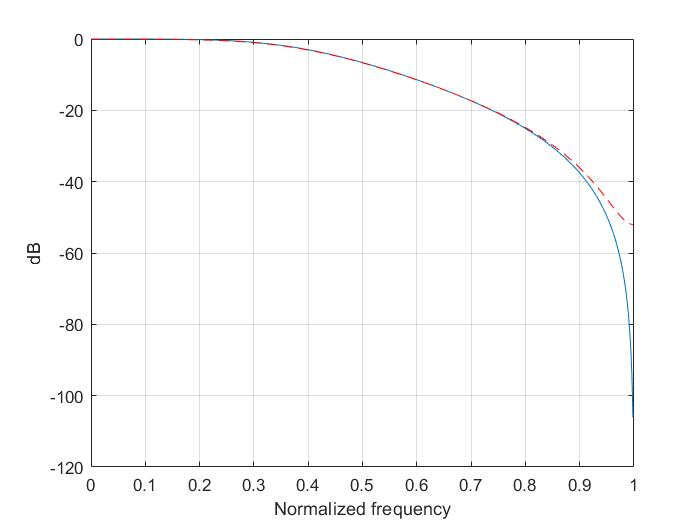
\includegraphics[width=8cm, height=6cm]{img/transfer_func.jpg} 
	\caption{IIR Transfer Function (Red is the quntized funcion).}
	\label{fig:IIR Transfer Function} 
\end{figure}

The function that implements this mechanism allows to save also the coefficients a and b as integers and as quantized parameters (ai, bi, aq, bq).

\begin{center}
    \begin{tabular}{ |c|c| } 
        \hline
            a_i & 256 -95 50\\
            \hline
            b_i & 52 105 52\\
            \hline
            a_q & 1 -0.3711 0.1953\\
            \hline
            b_q & 0.2031 0.4102 0.2031\\
        \hline
    \end{tabular}
    \begin{center}
    Tab. Outputs.
    \end{center}
\end{center}

\subsection{Filter Test}

To test the functioning of the filter, a signal was created consisting of two sinusoidal waves at two different frequencies, one in band with a frequency of 500 Hz and one out of band with a frequency of 4.5 KHz.\\
Using the obtained value (x) and the quantized parameters (aq, bq), generated by the IIR filter design function, as input to the Matlab "filter" function which allows to filter the input data x using a defined rational transfer function from the numerator and denominator coefficients bq and aq.\\
Below is an image depicting the two sinusoidal (x1, x2), the function input (\( x = \frac{x_1 + x_2}{2}\)) and the result of the filtering operation (y).

\begin{figure}[H]
	\centering
	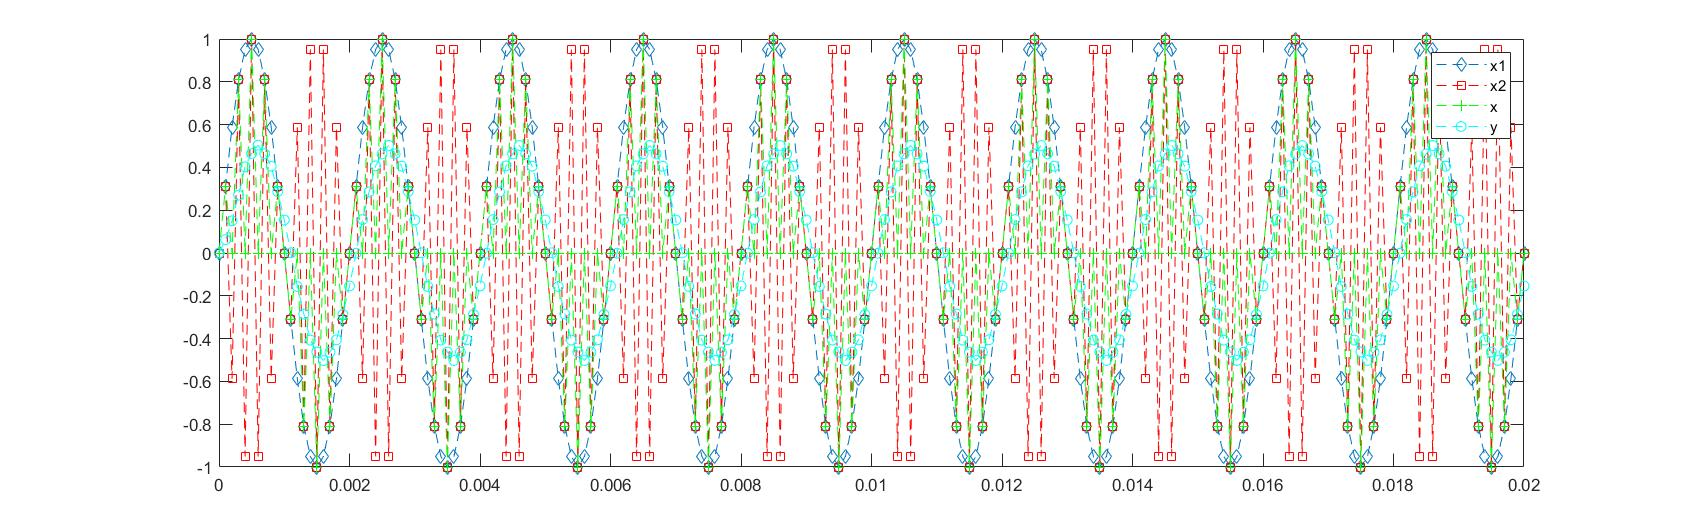
\includegraphics[width=\textwidth, height=6cm]{img/test.jpg} 
	\caption{Inputs and test result.}
	\label{fig:Inputs and test result} 
\end{figure}

In addition, the input and output samples are saved as quantized data represented on 9 bits as integer values, in two text files.\\
If we use the quantized output data to evaluate the total harmonic distortion we get a THD value equal to -52.53dB.\\
The graph is shown below.\\

\begin{figure}[H]
	\centering
	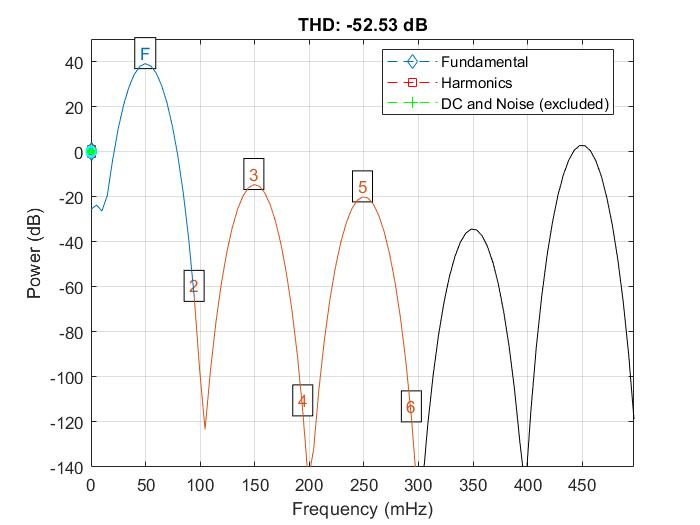
\includegraphics[width=\textwidth, height=6cm]{img/thdm.jpg} 
	\caption{THD of the Matlab model}
	\label{fig:THD} 
\end{figure}

\section{Fixed point C model}
In this section, a fixed-point model of the filtering operation is implemented through a program written in C.\\
This is done using the following formula:\\
\[\sum_{j} x_i_-_j * b_j - \sum_{k} y_i_-_k * a_k\]
Direct form II (canonical direct form) for IIR filters is used to implement this formula.\\
The program is able to cyclically read the input file generated by the Matlab model and calculate the filtered results. In order to do this, it uses a shift register and evaluates feed-back and feed-forward and the various intermediate values.\\
At the same time as reading, the program prints the results obtained in another file.\\
The code in order to emulate the behavior of the filter needs initial parameters to be fixed, such as:
\begin{itemize}
    \item Filter order
    \item Number of bits
    \item Coefficient \(b_0\) (first value of \(b_i\))
    \item b array (with the reaming 2 values of \(b_i\))
    \item a array (with the last 2 values of \(b_i\))
\end{itemize}

The program allows to reduce the number of bits after each multiplication, to reduce the bitwidth (and therefore the area) of the filter.\\

\subsection{THD}
Taking the output file of the fixed-point model made in C and on this data we can evaluate the THD.\\
The total harmonic distortion (THD) function allows to have the sinusoidal signal in dBc at real values passed to it.\\
The graph of the function is shown below.\\

\begin{figure}[H]
	\centering
	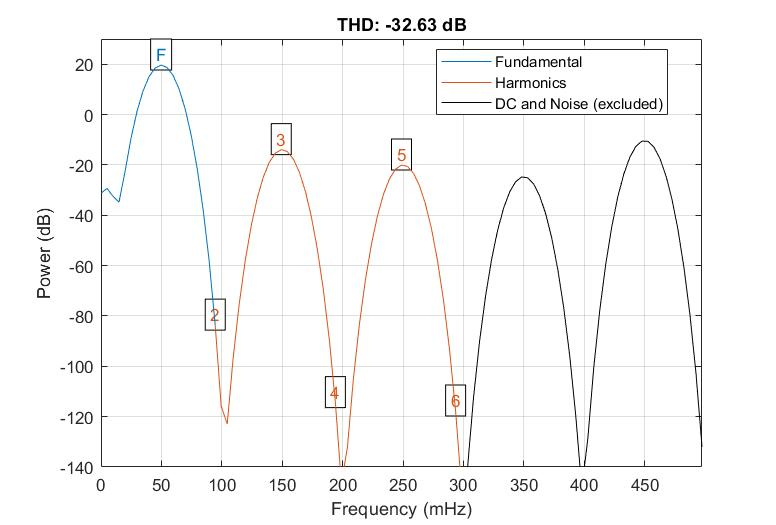
\includegraphics[width=\textwidth, height=6cm]{img/thdc.jpg} 
	\caption{THD of the fixed-point model}
	\label{fig:THD} 
\end{figure}

As you can see from the image, the THD value for this model is -32.63dB the is lower then -30dB that is the constraint.\\

\section{Comparison}

It can be seen that in the two models used we have different results.
This can be seen by directly analyzing the values present in the output files but also by looking at their THDs.\\
This is due to the fact that for the C model we are using fixed-point operators while the Matlab model uses floating point ones.\\